%%% 系统设计与实现

\section{开发环境与工具链}

\subsection{编程语言}

Juscan.jl库使用julia(version1.11.3)

\subsection{依赖库}

\begin{itemize}
  \setlength{\itemsep}{2pt}
  \item \lstinline|DataFrames.jl|: Julia基础数据框支持
  \item \lstinline|HDF5.jl|: 提供HDF5数据读写操作
  \item \lstinline|LinearAlgebra.jl|: Julia矩阵和线性代数库
  \item \lstinline|Loess.jl|: 回归平滑算法支持
  \item \lstinline|Muon.jl|: Muon.Anndata数据结构及基础行为
  \item \lstinline|SparseArrays.jl|: Julia稀疏矩阵支持
  \item \lstinline|Statistics.jl|, \lstinline|StatsBase.jl|: 基础统计学函数
  \item \lstinline|UMAP.jl|: 提供UMAP数据降维函数
\end{itemize}

\subsection{开发工具}

\begin{itemize}
  \setlength{\itemsep}{2pt}
  \item CPU: Intel i5-12500
  \item GPU: NVIDIA GeForce RTX 3050
  \item Platform:Arch Linux
  \item 单元测试:\lstinline|Test.jl|
  \item 调试器:\lstinline|Debugger.jl|
  \item 文档生成:\lstinline|Documenter.jl|
\end{itemize}

\section{Juscan.jl总体架构设计}

\subsection{整体流程图}

如图\ref{img:flow}所示,Juscan.jl的整体流程图展示了数据分析的主要步骤。首先,用户通过\lstinline|read_h5ad|函数读取HDF5格式的AnnData数据集。接着,数据预处理模块会计算质量控制指标,并根据用户设定的阈值进行细胞和基因过滤。随后,数据将被归一化处理,以消除测序深度差异带来的偏倚。最后,用户可以选择降维方法(如PCA或UMAP)进行数据可视化,并使用聚类算法(如Louvain或k-means)对细胞进行分群。

\begin{figure}[h]
  \centering
  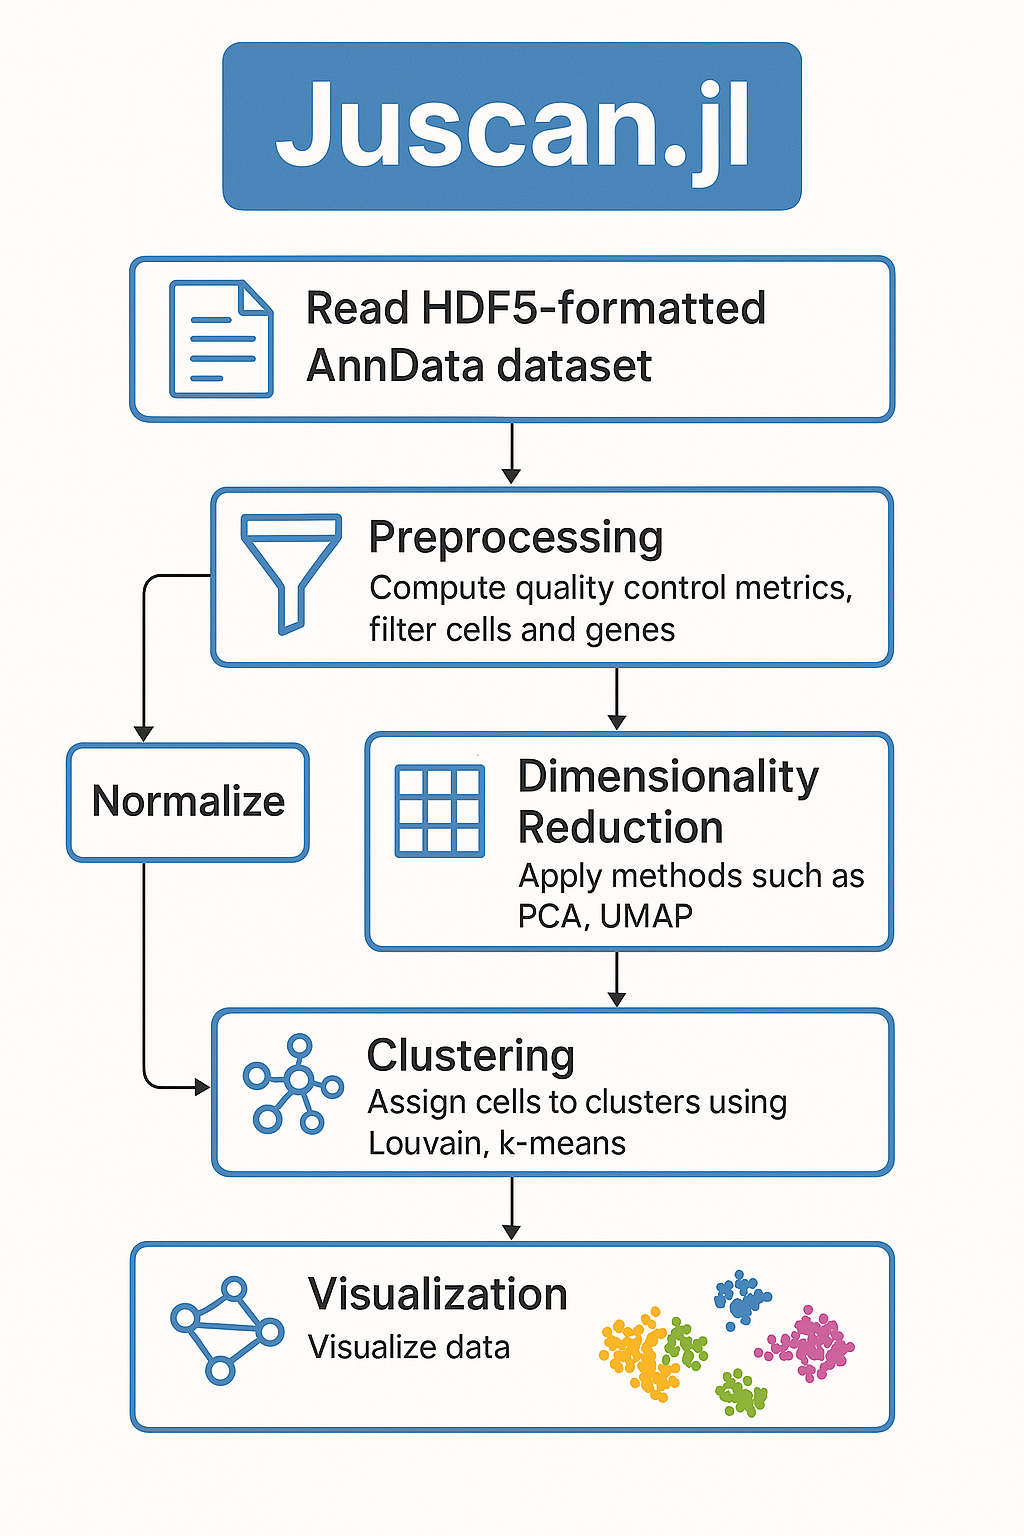
\includegraphics[width=0.4\textwidth]{img/flow_chart.png}
  \caption{Juscan.jl流程图}
  \label{img:flow}
\end{figure}

\subsection{系统模块划分}

如代码\ref{code:文件结构},此平台使用模块化的设计,将不同的功能划分到各自所属的模块中,以提高代码的整洁性、可维护性和扩展能力。

\begin{fancybox}{文件结构}
\addcontentsline{lot}{table}{代码~\thetcbcounter: 文件结构}
\begin{lstlisting}[numbers=none]
  Juscan.jl/
  ├── src/
  │   ├── preprocessing/
  │   │   ├── filter.jl                   # filter cells and genes
  │   │   ├── normalization.jl            # data normalization methods
  │   │   ├── pp.jl                       # preprocessing module
  │   │   ├── qc.jl                       # quality control methods
  │   │   └── utils.jl
  │   ├── tools/
  │   │   ├── cluster.jl                  # clustering methods
  │   │   ├── hvg.jl                      # highly variable genes
  │   │   ├── louvain.jl                  # louvain clustering
  │   │   ├── modularityClustering.jl     # modularity clustering
  │   │   ├── pca.jl                      # dimensionality reduction
  │   │   ├── snn.jl                      # SNN neighbour
  │   │   └── tl.jl                       # tools 
  │   ├── plots/
  │   │   ├── colors.jl
  │   │   ├── pl.jl
  │   │   └── plots.jl
  │   ├── Juscan.jl                       # Main module file
  │   ├── anndata.jl                      # anndata utilities
  │   └── utils.jl
  ├── docs/                               # documentation directory
  ├── test/                               # unit test directory
  ├── LICENSE
  ├── Project.toml                        # Julia project files
  └── README.md
\end{lstlisting}
\end{fancybox}

整体的Juscan.jl主要分为文档文件夹,单元测试文件夹,以及源代码文件夹。

源代码文件夹中Juscan.jl为整个项目的主模块,为项目导入需要的依赖库,加载子模块,以及对外暴露API接口。

导入的子模块包括preprocessing, tools, plots, 分别为单细胞的分析提供预处理,主要分析算法与可视化。

本项目由\href{https://github.com/scverse/Muon.jl}{Muon.jl}提供官方的AnnData数据结构, 代码\ref{code:Muon.AnnData}代表了Muon.anndata基本结构。

\section{数据结构}

\begin{fancybox}{Muon.AnnData}
\addcontentsline{lot}{table}{代码~\thetcbcounter: Muon.AnnData}
\begin{lstlisting}[language=julia]
mutable struct AnnData <: AbstractAnnData
  file::Union{HDF5.File, HDF5.Group, Nothing}

  X::Union{AbstractMatrix{<:Number}, Nothing}

  obs::DataFrame
  obs_names::Index{<:AbstractString}

  var::DataFrame
  var_names::Index{<:AbstractString}

  obsm::StrAlignedMapping{Tuple{1 => 1}, AnnData}
  obsp::StrAlignedMapping{Tuple{1 => 1, 2 => 1}, AnnData}

  varm::StrAlignedMapping{Tuple{1 => 2}, AnnData}
  varp::StrAlignedMapping{Tuple{1 => 2, 2 => 2}, AnnData}

  layers::AbstractAlignedMapping{Tuple{1 => 1, 2 => 2}, String}

  uns::Dict{<:AbstractString, <:Any}
end
\end{lstlisting}
\end{fancybox}

\begin{figure}[htbp]
  \centering
  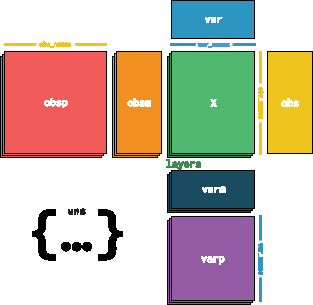
\includegraphics[width=0.5\textwidth]{img/anndata_schema.pdf}
  \caption{anndata数据结构示意图}
  \label{img:anndata}
\end{figure}


但是Muon.jl并没有提供足够多的处理anndata数据结构的方法行为,为了补充这方面的不足,本项目在\lstinline|src/anndata.jl|文件中进行了一些简单的扩充,包括子集化,插入观测与特征数据框,获取与设观测值的各个维度等方法。

\section{数据预处理模块}

\subsection{计算质量控制指标}

为了评估单细胞或多组学数据中的细胞与基因质量,我们实现了一个模块化的质量控制(quality control, QC)指标计算函数 \code{calculate_qc_metrics}。该函数支持从不同表达矩阵源(如主矩阵、原始计数矩阵 \code{adata.raw.X} 或指定的 \code{layer})提取表达数据,并分别计算细胞和基因层面的多种常用 QC 指标。

该函数的调用格式如下:

\begin{fancybox}{Muon.Pp.calculateQcMetrix}
\addcontentsline{lot}{table}{代码~\thetcbcounter: Muon.Pp.calculate\_qc\_metrix}
\begin{lstlisting}[language=julia]
calculate_qc_metrics(
  adata;
  expr_type="counts",
  var_type="genes",
  qc_vars=String[], 
  percent_top=[50, 100, 200, 500],
  layer=nothing,
  use_raw=false, 
  use_log1p=true,
  parallel=nothing
)::Tuple{DataFrame, DataFrame}
\end{lstlisting}
\end{fancybox}

在细胞维度上,函数会统计每个细胞中被检测到的特征数量、总表达量、log 转换后的表达水平、以及前若干高表达基因(如前 50、100、200 和 500 个)所占的表达比例。此外,用户可通过 \code{qc_vars} 参数指定一组具有特殊生物学意义的基因类别(如线粒体基因、核糖体基因等),函数将进一步评估这些类别基因在各细胞中的表达总量和比例。

在基因维度上,函数则计算每个基因在细胞群体中的检测频率、平均表达水平、零表达比例(dropout rate)以及总表达量等指标。这些指标可用于后续的基因过滤与特征选择。

函数 \code{calculate_qc_metrics} 返回两个 \code{DataFrame} 对象,分别包含细胞与基因层面的 QC 指标;而对应的 \code{calculate_qc_metrics!} 则为原地版本,直接将计算结果存储于 \code{adata.obs} 与 \code{adata.var} 字段中,便于与后续分析模块协同使用。

为支持灵活的数据接口设计,该模块还实现了表达矩阵的抽象选择函数 \code{_choose_mtx_rep},并对核心 QC 计算逻辑进行了进一步拆分,分别实现了用于细胞维度的 \code{describe_obs}/\code{describe_obs!} 和基因维度的 \code{describe_var}/\code{describe_var!}。其中,top-n 表达占比的计算由辅助函数 \code{top_segment_proportions} 实现。

该模块参考了 Scanpy 与 Seurat 的 QC 实践流程,并结合 Julia 类型系统设计了更高的通用性与可组合性,便于集成到多模态数据分析管线中。

\subsection{过滤}

在质量控制指标计算之后,我们进一步对数据进行细胞与基因的过滤,以剔除潜在的低质量条目,减少技术噪声对下游分析的干扰。本研究实现了一套通用的过滤函数,支持以总表达量、检测到的基因数(或细胞数)为阈值,灵活筛选细胞或基因,如代码\ref{code:Muon.Pp.filter}。

\begin{fancybox}{Muon.Pp.filter}
\addcontentsline{lot}{table}{代码~\thetcbcounter: Muon.Pp.filter}
\begin{lstlisting}[language=julia]
filter_cells!(
  data::Muon.AnnData;
  min_counts=nothing, min_genes=nothing,
  max_counts=nothing, max_genes=nothing
)::Nothing
filter_genes!(
  data::Muon.AnnData;
  min_counts=nothing, min_cells=nothing,
  max_counts=nothing, max_cells=nothing
)::Nothing
\end{lstlisting}
\end{fancybox}

细胞过滤函数 \code{filter_cells} 支持以下常用策略:

  \begin{itemize}
    \item 最小/最大总表达量(\code{min_counts}, \code{max_counts})
    \item 最小/最大检测基因数(\code{min_genes}, \code{max_genes})
    \item 可选择返回布尔向量(用于掩码子集)或过滤后的新对象(通过设置 \code{copy=true})
    \item 同时提供 \code{filter_cells!} 实现原地修改。
  \end{itemize}

类似地,基因过滤函数 \code{filter_genes} 支持以以下标准筛选:

  \begin{itemize}
    \item 被表达的细胞数量阈值(\code{min_cells}, \code{max_cells})
    \item 总表达量阈值(\code{min_counts}, \code{max_counts})
    \item 同样支持返回掩码或直接修改 \code{AnnData} 对象
  \end{itemize}

为确保操作语义明确,所有函数均要求每次仅传入一个过滤标准,以避免混淆。被筛选出的条目数量将在控制台输出日志,便于用户了解过滤效果。

该模块基于 Juscan.subset\_adata! 接口统一实现子集化操作,保证了代码的可维护性与高一致性,可无缝集成至数据预处理工作流中。

\subsection{归一化}


为消除不同细胞测序深度(即总 UMI 数)差异所带来的偏倚,我们实现了一个可扩展的总表达量归一化函数 \code{normalize_total},用于将每个细胞的表达矩阵缩放至统一的目标总量。该方法类似于 Scanpy 中的 \code{normalize_total} 或 Seurat 中的 \code{NormalizeData},但更具灵活性与模块化。

\begin{fancybox}{Muon.Pp.normalize}
\addcontentsline{lot}{table}{代码~\thetcbcounter: Muon.Pp.normalize}
\begin{lstlisting}
normalize_total(
    adata::AnnData;
    target_sum::Union{Real, Nothing}=nothing,
    exclude_highly_expressed::Bool=false,
    max_fraction::Float64=0.05,
    key_added::Union{String, Nothing}=nothing,
    layer::Union{String, Nothing}=nothing,
    layers::Union{String, Vector{String}, Nothing}=nothing,
    layer_norm::Union{String, Nothing}=nothing,
    copy::Bool=false
)::Union{AnnData, Dict{String, Any}}
normalize_total!(
    adata::AnnData;
    target_sum::Union{Real, Nothing}=nothing,
    exclude_highly_expressed::Bool=false,
    max_fraction::Float64=0.05,
    key_added::Union{String, Nothing}=nothing,
    layer::Union{String, Nothing}=nothing,
    layers::Union{String, Vector{String}, Nothing}=nothing
)::Nothing
\end{lstlisting}
\end{fancybox}

该函数通过计算每个细胞的总表达量(按行求和)作为归一化因子,并将表达矩阵按比例缩放,从而实现标准化。若未指定目标值(\code{target_sum}),则默认将每个细胞归一化至群体中位总表达量。此外,函数允许用户通过参数 \code{exclude_highly_expressed} 排除在某些细胞中高度表达的基因(如线粒体或核糖体基因),避免其对归一化因子的主导效应。

我们提供了两种版本的归一化函数:

    \code{normalize_total}:返回归一化后的新对象或结果字典;

    \code{normalize_total!}:原地(in-place)修改原始数据结构,节省内存。

这两个函数均支持对单个 \code{layer} 或多个 \code{layers} 进行归一化操作,并可通过参数 \code{layer_norm} 控制不同层归一化的参考因子。此外,归一化因子也可通过 \code{key_added} 参数保存至 \code{adata.obs} 中,用于后续批量分析或可视化。

值得注意的是,对于表达全为零的细胞,函数会发出警告提示。我们建议在归一化之前结合质量控制结果,先剔除此类无信息细胞。

\section{工具模块}

\subsection{高可变基因}

在单细胞 RNA 测序分析中,高变异基因(highly variable genes, HVGs)的识别对于后续的降维、聚类与轨迹推断等分析具有重要意义。为此,我们基于 Seurat v3 的策略,在 Julia 中实现了一套高变基因筛选模块 \code{highly_variable_genes},该方法兼容批次(batch-aware)处理,适用于多样本或多组学场景下的高变基因筛选。

该方法首先对每个批次独立计算每个基因的平均表达量与方差,并通过 LOESS 回归(局部加权多项式拟合)建模均值-方差关系,获得期望方差。随后,对原始方差进行校正,计算归一化后的方差作为变异性的衡量指标。对于跨多个批次的分析,方法进一步对各批次筛选结果进行合并,通过多批次中位排名的方式选出最终的一组 HVGs,保证其在多个批次中稳定地表现出高变异性。

我们实现了以下三类函数接口:

    % \code{highly_variable_genes}:返回 HVG 信息的 \code{DataFrame},不修改原始数据;
    % \code{highly_variable_genes!}:原地执行 HVG 计算,并将结果添加到 \code{adata.var};
    % \code{subset_to_hvg!}:在执行 HVG 筛选后,将数据集子集化,仅保留被识别为高变异的基因。
\begin{fancybox}{Muon.Tl.hvg}
\addcontentsline{lot}{table}{代码~\thetcbcounter: Muon.Tl.highly\_variable\_genes}
\begin{lstlisting}
subset_to_hvg!(adata::AnnData;
  layer::Union{String,Nothing} = nothing,
  n_top_genes::Int=2000,
  batch_key::Union{String,Nothing} = nothing,
  span::Float64=0.3,
  verbose::Bool=true
)
highly_variable_genes(adata::AnnData;
  layer::Union{String,Nothing} = nothing,
  n_top_genes::Int=2000,
  batch_key::Union{String,Nothing} = nothing,
  span::Float64=0.3
)
highly_variable_genes!(adata::AnnData;
  layer::Union{String,Nothing} = nothing,
  n_top_genes::Int=2000,
  batch_key::Union{String,Nothing} = nothing,
  span::Float64=0.3,
  replace_hvgs::Bool=true,
  verbose::Bool=false
)
\end{lstlisting}
\end{fancybox}

函数输出包括每个基因的均值、方差、归一化方差、在多个批次中的高变频次,以及最终的变异性排名。若数据中已有 HVG 注释,用户可选择是否替换(\code{replace_hvgs=true})。

\subsection{降维}

我们首先实现了 \code{log_transform!} 与 \code{logp1_transform!} 函数,用于对数据执行 $\log(x + \varepsilon)$ 或 $\log(1 + x)$ 变换,以增强表达量在低值区间的分布分辨能力。默认会将结果保存至新的数据层,便于复用与回溯。此外,函数 \code{standardize} 与 \code{prcomps} 封装了标准化与主成分提取过程,提供更底层的控制接口。

\subsubsection{(1)pca}

函数 \code{pca!} 实现了对 \code{AnnData} 对象中指定数据层的 PCA 计算,并将结果存储于 \code{adata.obsm["PCA"]} 中,供后续分析调用。该函数支持自动寻找合适的输入表达矩阵:若未提供目标数据层,则会依次查找是否存在经过对数转换的表达矩阵(\code{"log_transformed"})或归一化数据层(\code{"normalized"});若均不存在,则自动执行归一化与对数转换流程。

\begin{fancybox}{Muon.Tl.pca}
\addcontentsline{lot}{table}{代码~\thetcbcounter: Muon.Tl.pca}
\begin{lstlisting}
pca!(
  adata::Muon.AnnData;
  layer::String="log_transformed",
  n_pcs::Int=1000,
  verbose::Bool=true
)
\end{lstlisting}
\end{fancybox}

为确保主成分数量的合理性,函数会根据数据矩阵的维度自动调整主成分数量(\code{n_pcs}),避免维度溢出问题。计算过程采用稠密矩阵的奇异值分解(SVD)或稀疏矩阵的截断 SVD(TSVD),以兼容不同规模数据。

\subsubsection{(2)umap}

\begin{fancybox}{Muon.Tl.umap}
\addcontentsline{lot}{table}{代码~\thetcbcounter: Muon.Tl.umap}
\begin{lstlisting}
umap!(
  adata::Muon.AnnData;
  layer::String="log_transformed",
  use_pca_init::Bool=false,
  n_pcs::Int=100,
  verbose::Bool=true,
  kwargs...
)
\end{lstlisting}
\end{fancybox}

函数 \code{umap!} 用于计算数据的 UMAP 嵌入,并将结果包括嵌入坐标、最近邻索引、距离矩阵与模糊邻接图分别存入 \code{adata.obsm} 与 \code{adata.obsp} 中。该函数支持两种初始化方式:

\begin{itemize}
  \item 直接嵌入:使用指定数据层或自动生成的对数转换数据
  \item PCA 初始化:通过设置 \code{use_pca_init=true},先执行 PCA 作为初始嵌入向量
\end{itemize}

UMAP本身使用\code{UMAP.jl}实现,默认基于余弦距离构建邻接图,并可通过传入关键字参数(如 \code{n_neighbors}, \code{min_dist} 等)实现参数化控制。

\subsection{聚类}

聚类分析是单细胞数据中识别细胞亚群结构的关键步骤。此部分代码部分参考\code{ASCT.jl}的实现方法\upcite{Yang2023.12.27.573479}, 对\code{Muon:Ammdata}数据结构进行两类聚类方法:图结构驱动的模块度聚类(modularity clustering)与基于中心点的 KMedoids 聚类(近似 KMeans),构成了双路径的细胞聚类框架。为了便于用户在不同分析阶段调用聚类方法,我们提供了统一接口 clustering!,支持多种参数配置与算法选择。

\begin{fancybox}{Muon.Tl.Clustering}
\addcontentsline{lot}{table}{代码~\thetcbcounter: Juscan.Tl.Clustering}
  \begin{lstlisting}
function clustering!(
  data::Muon.AnnData;
  method::AbstractString="mc",
  reduction::Union{AbstractString, Symbol}=:auto,
  use_pca::Union{AbstractString, Integer}="pca_cut",
  # n_pcs::Union{Integer, AbstractString}=5,
  tree_K::Integer=20,
  resolution::Union{Symbol, Real, AbstractRange}=:auto,
  cluster_K::Union{Nothing, Integer}=nothing,
  cluster_K_max::Union{Nothing, Integer}=30,
  dist::AbstractString="Euclidean",
  network::AbstractString="SNN",
  random_starts_number::Integer=10,
  iter_number::Integer=10,
  prune::AbstractFloat=1 / 15,
  seed::Integer=-1,
)
  \end{lstlisting}
\end{fancybox}

对\code{AnnData}对象执行聚类分析,结果会自动保存在\code{adata.obs}中。该函数根据参数\code{method}选择不同的聚类策略。

\textbf{a.~基于模块度的图聚类(modularity clustering)}

该方法通过构建细胞的共享最近邻图(Shared Nearest Neighbor, SNN),并以最大化模块度(modularity)为目标,对细胞图进行社团划分。方法流程如下:

\begin{enumerate}
  \item 图构建:在降维空间(如 PCA)中,使用 KD 树加速寻找每个细胞的 $K$ 个近邻,构建 KNN 或 SNN 图。SNN 图定义如下:

\begin{equation}
  \text{SNN}_{ij} = |\mathcal{N}_i \cap \mathcal{N}_j| / K
\end{equation}

其中 $\mathcal{N}_i$ 表示细胞 $i$ 的邻居集合。

\item 图稀疏化与剪枝:通过阈值参数 $\alpha \in (0, 1]$ 对图进行稀疏化,仅保留重叠度高的邻接关系,以提高模块度检测的稳定性。

\item 模块度优化聚类:通过 Louvain 或 Leiden 等算法,在图中最大化以下模块度函数:

\begin{equation}
Q = \frac{1}{2m} \sum_{i,j} \left( A_{ij} - \gamma \frac{k_i k_j}{2m} \right) \delta(c_i, c_j)
\end{equation}

其中 $A_{ij}$ 为图邻接矩阵,$k_i$ 为节点度,$\gamma$ 为分辨率参数,$\delta$ 为 Kronecker delta。我们支持不同的 $\gamma$ 参数进行多分辨率扫描,自动推荐最优分辨率。

\end{enumerate}

\textbf{b.~基于KMedoids的中心点聚类(k-medoids clustering)}

KMedoids 聚类是一种鲁棒于异常值的变体,相较于 KMeans 选择“簇中心”,KMedoids 选择实际数据点作为中心。我们实现如下自动聚类过程:

\begin{enumerate}
  \item 距离计算:用户可选择多种距离度量,如欧氏距离、余弦距离、相关距离等,在降维空间中计算细胞间距离矩阵。

  \item 自动选择簇数 $K$:

  \begin{itemize}
    \item 计算多个 $K$ 值下的聚类结果(并行加速);
    \item 对每个聚类结果,计算 silhouette 系数 $\bar{s}$ 与标准差;
    \item 同时评估总成本的肘部法则(elbow method);
    \item 综合两个指标,自动选择最优 $K$ 值:
  \end{itemize}

\end{enumerate}

\begin{equation}
K^* = \arg\max_K \left( \text{silhouette score} - \text{total cost deviation} \right)
\end{equation}

\section{可视化模块}

单细胞组学分析常涉及高维数据的降维、聚类和分类结果,为了更好地呈现这些复杂结构,我们在 \code{Juscan.Plots} 中实现了一套基于 \code{CairoMakie} 的绘图模块,涵盖多种用于探索性分析与结果展示的图形函数。该模块强调高可配置性、视觉一致性与图像质量,便于科研报告与论文作图。

\subsection{调色机制与主题色板}

我们设计了一套模块化的调色系统,通过 \code{get_palette} 和 \code{get_continuous_colormap} 接口,提供一系列离散与连续的调色方案,支持自动扩展与下采样。其中,离散色板如 \code{"friendly"}、\code{"apple"}、\code{"rainbow"} 等适用于类别标签着色,而连续色带则集成自 \code{ColorSchemes.jl},可用于表达量、主成分值等数值信息的可视化。所有色板均通过自定义函数实现扩展与裁剪策略,确保图形风格在多图展示中保持一致。

\subsection{可视化函数接口}

模块当前提供以下核心函数:

\begin{itemize} \item \code{violin}:绘制提琴图,展示多个观测变量(如基因表达、细胞指标)的分布,支持点抖动(jitter)与多子图并排布局。 \item \code{scatter}:绘制二维散点图,支持根据第三变量进行着色(如根据表达量、UMAP/PCA位置等变量上色)。 \item \code{hvg_scatter}:用于展示高变异基因的筛选结果,通过平均表达与变异度关系图突出高变基因在全体中的位置。 \item \code{plot_variance_ratio}:绘制 PCA 主成分的方差解释比例图,支持对前若干主成分进行可视化,并自动标注前 5 个 PC。 \item \code{plot_umap}:绘制 UMAP 降维嵌入图,支持按照类别标签上色,自动生成图例并匹配色板风格。 \end{itemize}

\subsubsection{(1) violin:分布可视化}

该函数支持绘制多个变量在样本中的表达分布,可用于细胞质控指标(如总 UMI 数、线粒体比例)的展示。用户可指定色板名与透明度参数,自动匹配子图数量与调色方案。此外还可设置点抖动强度与保存图像路径:

\begin{fancybox}{Juscan.Plots.violin} 
  \addcontentsline{lot}{table}{代码~\thetcbcounter: Muon.Pl.violin}
  \begin{lstlisting} 
violin(
  adata::AnnData,
  keys::Union{String, Vector{String}};
  width::Real=600,
  height::Real=400,
  jitter::Union{Bool, Real}=0.5, dot_size::Real=2,
  title::String="violin plot",
  palette_name::String="friendly",
  fill_alpha::Real=1.0, 
  savefig::Union{Bool, String}=false
) 
  \end{lstlisting} 
\end{fancybox}

\subsubsection{(2) hvg\_scatter:高变基因展示}

为辅助用户评估 HVG 的筛选结果,我们实现了 \code{hvg_scatter} 函数,绘制均值-方差与归一化方差的二维图。灰色表示非 HVG 基因,黑色点表示已筛选出的 HVGs,有助于观察其在全体中的分布位置。

\subsubsection{(3) plot\_umap:嵌入可视化}

该函数根据 \code{adata.obsm} 中的 UMAP 坐标绘图,并根据 \code{adata.obs} 中的分类变量进行着色。支持自定义调色板、图形尺寸与图像保存路径:

\begin{fancybox}{Juscan.Plots.plot umap}
  \addcontentsline{lot}{table}{代码~\thetcbcounter: Muon.Pl.plot\_umap}
  \begin{lstlisting} 
plot_umap(
  adata;
  color_by::String="clusters_latest",
  key="umap",
  palette_name::String="rainbow",
  savefig::Union{Bool, String}=false
) 
  \end{lstlisting} 
\end{fancybox}

\subsubsection{(4) scatter 与 plot\_variance\_ratio}

除标准二维散点图外,我们也实现了用于主成分方差比分析的函数 \code{plot_variance_ratio}。其通过绘制 log 方差比图,帮助用户直观判断 PCA 的有效维度。
